\begin{abstract}
Knowledge distillation (KD) has historically served as the primary vehicle for model compression, transferring capabilities from massive teacher models to efficient student architectures. However, the advent of Large Language Models (LLMs) has catalyzed a fundamental paradigm shift from static, off-policy distillation to On-Policy Distillation (OPD). In this survey, we provide a comprehensive and theoretically grounded overview of OPD. We posit a core insight that must govern the modern understanding of distillation: the essence of OPD is not merely a choice of divergence metrics, but a profound paradigm shift in \textit{"who decides the training distribution."} By allowing the student's own generative manifold to dictate the state distribution, OPD directly mitigates the catastrophic train-test mismatch and compounding exposure bias inherent in autoregressive decoding. 
We systematically taxonomize the field into three converging trajectories based on feedback signals: Logit-based, Outcome-based, and Self-play methodologies. Furthermore, we critically analyze frequently neglected dimensions, including the compute-quality tradeoff, the teacher's "echo chamber" in uncertain regions, dynamic divergence adaptation, and the conceptualization of distillation as structured knowledge transfer rather than mere compression. Finally, we map out pivotal future directions, from distillation scaling laws to agent-level OPD.
\end{abstract}

\section{Introduction}
\label{sec:intro}

The rapid evolution of Large Language Models (LLMs) has continuously pushed the boundaries of artificial intelligence, achieving remarkable milestones in natural language understanding, reasoning, and generation. However, the massive parameter counts of frontier models pose severe constraints on deployment, inference latency, and energy efficiency. Recently, the open-source community witnessed a monumental milestone: the DeepSeek-R1 model \citep{2501.12948} successfully distilled the profound, complex reasoning capabilities of a 671-billion parameter Mixture-of-Experts (MoE) model into dense models as small as 7 billion parameters. This spectacular success underscores a vital reality—knowledge distillation is no longer a marginal optimization technique used merely for slight latency improvements; it is the central engine for democratizing cutting-edge intelligence and creating highly capable, specialized models that can operate on consumer-grade hardware. The urgency to systematically understand, theoretically formalize, and algorithmically advance LLM distillation has never been greater.

Traditionally, distillation in Natural Language Processing has been heavily dominated by off-policy methods. In this standard paradigm, a student model is trained to mimic a teacher's token-level probabilities over a fixed, static dataset drawn from the data distribution $\pdata$. However, as elegantly illuminated by studies investigating the "false promise" of imitating proprietary LLMs \citep{2305.15717}, off-policy distillation suffers from a fatal, fundamental flaw: \textit{train-test mismatch}. During training, the student is strictly conditioned on gold-standard prefixes from the fixed dataset, a technique known as teacher-forcing. During inference, however, the student must condition on its own previously generated tokens in an autoregressive manner. When the student inevitably makes a minor error and deviates from the optimal path, it enters out-of-distribution (OOD) territory where it has received absolutely no supervisory signal during training. This lack of guidance leads to a cascade of subsequent errors—a compounding phenomenon formally known in the literature as \textit{exposure bias}. 

To bridge this massive chasm, the field is rapidly migrating towards \textbf{On-Policy Distillation (OPD)}. Drawing deep conceptual linkages with Imitation Learning, specifically the DAgger (Dataset Aggregation) algorithm introduced by \citet{ross2011reduction}, OPD forces the student model to generate trajectories according to its own current policy ($\pi_\theta$). The algorithm then selectively queries the teacher to provide feedback, logits, or rewards on these student-generated paths. We posit the following central thesis for this survey:
\textbf{Core Insight:} \textit{The true essence of On-Policy Distillation is not simply the mathematical choice of probability divergence (e.g., Forward KL versus Reverse KL), but rather a profound paradigm shift in "who decides the training distribution."} The transition from $y \sim \pdata$ to $y \sim \ptheta$ fundamentally transforms the learning objective from memorizing an alien, unattainable distribution to optimally navigating and correcting the student's own reachable generative manifold.

Despite the explosive growth of OPD methodologies in recent months—ranging from Generalized Knowledge Distillation (GKD) \citep{2306.13649} to MiniLLM \citep{2306.08543} and self-play mechanisms like SPIN \citep{2401.01335}—the literature remains highly fragmented. Current surveys, such as the comprehensive overview by \citet{2402.13116}, primarily treat distillation as a monolithic model compression step. While valuable, they lack a rigorous, unified mathematical perspective on the complex on-policy dynamics that govern modern LLM alignment and reasoning transfer. This paper directly addresses this critical gap by dissecting the mathematical foundations, categorizing the emerging algorithmic variants into a cohesive taxonomy, and spotlighting the severe blind spots of current research.

Specifically, the contributions of this comprehensive review are formally encapsulated in the following five dimensions:
\begin{itemize}
    \item \textbf{A Unified Theoretical Framework:} We rigorously formulate the transition from classical off-policy to modern on-policy distillation, mapping it directly to sequential decision-making and f-divergence minimization. This framework mathematically unifies disparate seminal works, demonstrating how methods like GKD \citep{2306.13649}, MiniLLM \citep{2306.08543}, and DistiLLM \citep{2402.03898} are essentially optimizing the same underlying objective under different divergence constraints and sampling mixtures.
    \item \textbf{A Novel, Feedback-Centric Taxonomy:} We systematically categorize the sprawling OPD landscape into three primary technical routes based on the nature of the supervisory signal: \textit{Logit-based} approaches (computationally dense but requiring white-box access), \textit{Outcome-based} approaches (sparse but highly flexible, often utilizing Process Reward Models as seen in \citet{2305.20050}), and \textit{Self-play} approaches (teacher-free but prone to rapid performance saturation). We further highlight how these traditionally isolated tracks are actively converging into hybrid methodologies, such as AlignDistil \citep{2503.02832} and MiMo-V2 \citep{2601.02780}.
    \item \textbf{Identification of Neglected Critical Issues:} We bring to light fundamental theoretical and empirical challenges that the community has largely ignored. These include: (a) The missing systematic analysis of the \textit{compute-quality tradeoff} in online distillation, where the cost of generating on-policy data often outweighs the distillation benefits; (b) The "echo chamber" effect, where querying teachers in regions of extreme student uncertainty leads to misaligned, high-variance gradients; (c) The urgent necessity for \textit{dynamic divergence adaptation} rather than static KL metric selection; and (d) Reconceptualizing distillation as \textit{structured knowledge transfer} rather than mere parameter compression.
    \item \textbf{Bridging the White-box and Black-box Divide:} We provide an exhaustive analysis of how on-policy techniques adapt when internal teacher states are inaccessible. By comparing exact logit matching methods with API-driven outcome matching frameworks like Lion \citep{2310.01382} and GAD \citep{2511.10643}, we reveal the theoretical bounds of what can be learned strictly from top-1 generations versus full probability distributions.
    \item \textbf{Roadmap for Future Directions:} We strategically chart the unexplored territories of LLM distillation, detailing the mathematical necessity for robust distillation scaling laws, the potential of uncertainty-aware OPD, and the inevitable shift towards agent-level environmental distillation where models learn from multi-turn, state-dependent interactions rather than static text completions.
\end{itemize}

The remainder of this survey is meticulously organized to build from fundamental theories to state-of-the-art applications. Section~\ref{sec:background} establishes the strict mathematical preliminaries, formalizing exposure bias, sequence-level cross-entropy, and the f-divergence family. Section~\ref{sec:taxonomy} presents our novel, comprehensive taxonomy of OPD methodologies, complete with a visual structural breakdown. Subsequent sections will systematically dissect logit-based optimization, outcome-reward architectures, advanced reasoning distillation, and ultimately conclude with an analysis of open challenges and future trajectories.


\section{Background and Preliminaries}
\label{sec:background}

To rigorously appreciate the monumental leap from standard, dataset-bound Knowledge Distillation to dynamic On-Policy Distillation, we must first establish a strict formalization of the sequential nature of LLM generation. This section provides deep mathematical definitions of distribution matching, formalizes the exposure bias phenomenon, and constructs a unified mathematical framework utilizing the f-divergence family.

\subsection{Knowledge Distillation Fundamentals}
\label{subsec:kd_fundamentals}

The classical Knowledge Distillation framework, originally pioneered by \citet{hinton2015distilling}, was designed to transfer the implicit "dark knowledge" embedded within the continuous probability distributions of a cumbersome teacher network $\mathcal{T}$ to a more compact student network $\mathcal{S}$. In standard classification tasks, and by extension, token-level vocabulary selection in language modeling, a neural network produces a vector of pre-softmax logits $z \in \mathbb{R}^{|V|}$, where $|V|$ is the dimensionality of the vocabulary. 

To extract the relational structure between distinct classes—for instance, understanding that the token "automobile" is semantically much closer to "car" than to "apple"—the logits are smoothed utilizing a temperature scalar $\tau > 0$. The softened probability distribution for a given input context $x$ is formally defined by the modified softmax function:
\begin{equation}
    P(y|x; \tau) = \frac{\exp(z_y / \tau)}{\sum_{y' \in V} \exp(z_{y'} / \tau)}
\end{equation}
The standard KD objective seeks to minimize the Kullback-Leibler (KL) divergence between the teacher's softened predictive distribution $\pteacher$ and the student's corresponding softened distribution $\ptheta$:
\begin{equation}
    \loss_{\mathrm{KD}} = \tau^2 \KL(\pteacher(\cdot|x; \tau) \parallel \ptheta(\cdot|x; \tau)) = \tau^2 \sum_{y \in V} \pteacher(y|x; \tau) \log \left( \frac{\pteacher(y|x; \tau)}{\ptheta(y|x; \tau)} \right)
\end{equation}
The $\tau^2$ scaling factor is of paramount mathematical importance. As $\tau$ increases, the magnitudes of the gradients produced by the cross-entropy loss scale down by a factor of $1/\tau^2$. Therefore, multiplying the objective by $\tau^2$ ensures that the relative contribution of the distillation loss remains commensurate with standard hard-label cross-entropy loss when combined in a joint training objective. 

To understand the deep mechanics of this transfer, we can analyze the gradient of the distillation loss with respect to the student's logits $z_i^{\mathcal{S}}$. Let $p_i^{\mathcal{T}}$ and $p_i^{\mathcal{S}}$ denote the temperature-scaled probabilities for the teacher and student, respectively. The gradient is simply:
\begin{equation}
    \frac{\partial \loss_{\mathrm{KD}}}{\partial z_i^{\mathcal{S}}} = \frac{\tau^2}{\tau} (p_i^{\mathcal{S}} - p_i^{\mathcal{T}}) = \tau (p_i^{\mathcal{S}} - p_i^{\mathcal{T}})
\end{equation}
When the temperature $\tau \to \infty$, we can apply a Taylor expansion to the exponential terms, $\exp(z_i/\tau) \approx 1 + z_i/\tau$. Assuming the logits have been zero-meaned ($\sum_j z_j = 0$), the probabilities asymptotically approach:
\begin{equation}
    p_i \approx \frac{1 + z_i/\tau}{|V| + \sum_j z_j/\tau} = \frac{1}{|V|} + \frac{z_i}{|V|\tau}
\end{equation}
Substituting this back into the gradient equation reveals a profound equivalence:
\begin{equation}
    \frac{\partial \loss_{\mathrm{KD}}}{\partial z_i^{\mathcal{S}}} \approx \tau \left( \frac{z_i^{\mathcal{S}}}{|V|\tau} - \frac{z_i^{\mathcal{T}}}{|V|\tau} \right) = \frac{1}{|V|} (z_i^{\mathcal{S}} - z_i^{\mathcal{T}})
\end{equation}
This derivation mathematically proves that in the high-temperature limit, classical knowledge distillation perfectly degenerates into minimizing the Mean Squared Error (MSE) between the teacher's and student's raw logits. This behavior forces the student to holistically replicate the teacher's entire internal logit landscape, transferring both the primary predictive modes and the nuanced, sub-optimal probability masses (the dark knowledge) that dictate the teacher's generalization capabilities. However, when applied naively to autoregressive LLMs, this formulation heavily assumes that the input $x$ (the prefix) is perfectly drawn from the target data distribution, entirely ignoring the sequential, compounding nature of language generation.

\subsection{Token-Level vs. Sequence-Level Distillation}
\label{subsec:token_vs_sequence}

The direct application of \citet{hinton2015distilling}'s formulation to language modeling typically manifests as token-level distillation. In an autoregressive setting, a sequence $y = (y_1, y_2, \dots, y_T)$ is generated conditionally. Let $y_{<t}$ denote the prefix up to step $t$. The token-level cross-entropy distillation loss is expressed as the expected divergence over prefixes drawn from the empirical dataset $\mathcal{D}$:
\begin{equation}
    \loss_{\mathrm{Token-KD}} = \mathbb{E}_{x, y \sim \mathcal{D}} \left[ \sum_{t=1}^{|y|} \KL(\pteacher(\cdot | x, y_{<t}) \parallel \ptheta(\cdot | x, y_{<t})) \right]
\end{equation}
While computationally tractable because it relies on static, pre-computed prefixes, token-level KD fundamentally misaligns with the global generative objective. It optimizes the student's next-token accuracy while assuming the history $y_{<t}$ is perfectly error-free. 

Recognizing this critical limitation, \citet{kim2016sequence} proposed Sequence-Level Knowledge Distillation. Instead of factorizing the loss token-by-token over fixed dataset prefixes, sequence-level KD aims to match the joint probability distributions over the entire sequence space $\mathcal{Y}$. The theoretical sequence-level objective minimizes the global KL divergence:
\begin{equation}
    \loss_{\mathrm{Seq-KD}} = \KL(P_{\mathcal{T}}(y | x) \parallel P_{\theta}(y | x)) = \sum_{y \in \mathcal{Y}} P_{\mathcal{T}}(y | x) \log \left( \frac{P_{\mathcal{T}}(y | x)}{P_{\theta}(y | x)} \right)
\end{equation}
Because the space of all possible sequences $\mathcal{Y}$ grows exponentially with the sequence length $T$ (i.e., $|\mathcal{Y}| = |V|^T$), exactly computing this summation is strictly intractable. To resolve this, \citet{kim2016sequence} introduced a pragmatic approximation. By observing that the teacher's distribution $P_{\mathcal{T}}(y|x)$ is heavily peaked around its mode, they approximated the distribution with a Dirac delta function centered on the sequence generated by performing beam search on the teacher:
\begin{equation}
    P_{\mathcal{T}}(y | x) \approx \begin{cases} 
      1 & \text{if } y = \arg\max_{y' \in \mathcal{Y}} P_{\mathcal{T}}(y' | x) \\
      0 & \text{otherwise} 
   \end{cases}
\end{equation}
By substituting this approximation back into the sequence-level KL divergence, the loss elegantly collapses to the standard negative log-likelihood (NLL) of the student model, evaluated exclusively on the teacher's highest-probability sequence, $\hat{y}$:
\begin{equation}
    \loss_{\mathrm{Seq-Approx}} = - \sum_{t=1}^{|\hat{y}|} \log \ptheta(\hat{y}_t | x, \hat{y}_{<t})
\end{equation}
This formulation represents a critical conceptual leap: it forces the student to model complete trajectories that are highly favored by the teacher, implicitly transferring sequence-level structural dependencies. However, from a rigorous theoretical standpoint, Sequence-Level KD remains an \textit{off-policy} algorithm. The student is still trained via teacher-forcing on static trajectories—in this case, pseudo-labels generated offline by the teacher. While the target sequence $\hat{y}$ is generated by a model rather than a human, the student during training never conditions its predictions on its own generated prefixes. Consequently, Sequence-Level KD, despite its mathematical elegance, remains deeply susceptible to the very train-test mismatch it sought to alleviate, laying the precise groundwork for the necessity of true on-policy algorithms.

\subsection{The Distribution Mismatch Problem and Exposure Bias}
\label{subsec:exposure_bias}

The fundamental pathology that necessitates On-Policy Distillation is formally defined as \textit{exposure bias}, a direct manifestation of covariate shift in sequential decision-making. To rigorously articulate this, we must cast autoregressive generation as a Markov Decision Process (MDP). Let the state space $\mathcal{S}$ be the set of all possible token prefixes $s_t = (x, y_{<t})$, and the action space $\mathcal{A}$ be the vocabulary $V$. The transition dynamics are strictly deterministic: taking action $y_t$ in state $s_t$ deterministically leads to state $s_{t+1} = (x, y_{<t}, y_t)$. 

During standard off-policy distillation (teacher-forcing), the states encountered by the student are rigorously governed by the data distribution $\pdata$. Let us define the state visitation distribution under the dataset policy as $d_{\pdata}(s)$. The training objective is an expectation over this specific distribution:
\begin{equation}
    \loss_{\mathrm{train}} = \mathbb{E}_{s \sim d_{\pdata}} \left[ \KL(\pteacher(\cdot|s) \parallel \pi_\theta(\cdot|s)) \right]
\end{equation}
During inference, however, the student model must act according to its own learned policy $\pi_\theta$. Because the student is imperfect, its actions will inevitably deviate from the dataset distribution. Let $d_{\ptheta}(s)$ denote the state visitation distribution induced when the student rolls out its own trajectories. The testing objective (or true generation quality) is evaluated under this distinct distribution:
\begin{equation}
    \loss_{\mathrm{test}} = \mathbb{E}_{s \sim d_{\ptheta}} \left[ \loss_{\mathrm{task}}(s, \pi_\theta) \right]
\end{equation}
The exposure bias problem is defined by the inequality of these distributions: $d_{\pdata}(s) \neq d_{\ptheta}(s)$. Because the student was never exposed to the states in the support of $d_{\ptheta}(s) \setminus d_{\pdata}(s)$ during training, it receives zero supervisory signal in these regions. 

We can quantify the severity of this mismatch using formal performance bounds derived from Imitation Learning. As demonstrated by the seminal DAgger analysis by \citet{ross2011reduction}, if a student policy $\pi_\theta$ is trained to mimic a teacher policy $\pi^*$ such that the expected error at each time step under the training distribution is bounded by $\epsilon$, i.e., $\mathbb{E}_{s \sim d_{\pi^*}}[\mathbb{I}(\pi_\theta(s) \neq \pi^*(s))] \le \epsilon$, then the expected total discrepancy over a trajectory of length $T$ under the student's own induced distribution scales quadratically:
\begin{equation}
    \mathbb{E}_{s \sim d_{\ptheta}} \left[ \sum_{t=1}^T \loss(s_t) \right] \le O(\epsilon T^2)
\end{equation}
This $O(T^2)$ compounding error bound is catastrophic for modern LLMs, which routinely generate sequences spanning thousands of tokens. A single suboptimal token choice shifts the prefix slightly out-of-distribution; the model, having never seen this perturbed prefix, is more likely to make a second error, rapidly spiraling into hallucinatory or structurally compromised text. On-Policy Distillation resolves this by fundamentally altering the expectation operator in the training objective from $\mathbb{E}_{s \sim d_{\pdata}}$ to $\mathbb{E}_{s \sim d_{\ptheta}}$. By generating responses online, the student is forced to confront its own mistakes, receive teacher feedback on those specific out-of-distribution states, and learn robust recovery behaviors, effectively reducing the error accumulation from $O(T^2)$ back to $O(\epsilon T)$.

\subsection{The f-Divergence Family and Geometric Intuition}
\label{subsec:f_divergence}

To parameterize the precise nature of the distribution matching in OPD, we rely on the f-divergence framework. Given two probability distributions $P$ and $Q$ over a continuous or discrete space $\mathcal{X}$, an f-divergence is a strictly convex function that measures the discrepancy between them. For any convex function $f: (0, \infty) \to \mathbb{R}$ such that $f(1) = 0$, the f-divergence is formally defined as:
\begin{equation}
    D_f(P \parallel Q) = \int_{\mathcal{X}} Q(x) f\left(\frac{P(x)}{Q(x)}\right) dx = \mathbb{E}_{x \sim Q} \left[ f\left(\frac{P(x)}{Q(x)}\right) \right]
\end{equation}
The choice of the generating function $f(u)$ yields vastly different geometrical properties for the resulting distillation objective. In the context of LLMs, where $P$ is typically the complex, multi-modal teacher distribution $\pteacher$ and $Q$ is the highly constrained, lower-capacity student distribution $\ptheta$, understanding these geometries is paramount.

\textbf{1. Forward Kullback-Leibler Divergence:} By selecting $f(u) = u \log u$, we recover the Forward KL divergence, $D_{\mathrm{KL}}(P \parallel Q) = \mathbb{E}_{x \sim P} [ \log(P(x)/Q(x)) ]$. The gradient forces the student $Q$ to place probability mass everywhere the teacher $P$ has mass. If there exists a region where $P(x) > 0$ but $Q(x) \approx 0$, the penalty approaches infinity. Consequently, Forward KL is strongly \textit{mode-covering} (or zero-avoiding). In LLM distillation, because a small student lacks the capacity to memorize the vast, diverse linguistic distribution of a massive teacher, attempting to cover all modes often results in the student placing probability mass in the void between valid modes, leading to the generation of nonsensical, average phrasing.

\textbf{2. Reverse Kullback-Leibler Divergence:} By selecting $f(u) = -\log u$, we recover the Reverse KL divergence, $D_{\mathrm{KL}}(Q \parallel P) = \mathbb{E}_{x \sim Q} [ \log(Q(x)/P(x)) ]$. Here, the expectation is taken with respect to the student $Q$. If the student places mass $Q(x) > 0$ in a region where the teacher $P(x) \approx 0$, the penalty is infinite. To minimize this, the student ensures it only assigns probability to regions explicitly supported by the teacher. This leads to a \textit{mode-seeking} (or zero-forcing) behavior. The student will gracefully collapse its distribution onto one major, highly probable mode of the teacher, completely ignoring minor modes. For generative language, this is highly desirable, as producing one coherent, correct answer is infinitely preferable to generating an incoherent amalgamation of multiple correct answers.

\textbf{3. Jensen-Shannon Divergence (JSD):} JSD introduces symmetry by measuring the divergence to a mixture distribution $M = \frac{1}{2}(P + Q)$. Utilizing $f(u) = u \log\left(\frac{2u}{u+1}\right) + \log\left(\frac{2}{u+1}\right)$, the formulation is bounded between 0 and $\log 2$, offering a highly stable gradient landscape that balances both mode-seeking and mode-covering properties, preventing extreme gradient explosions in out-of-distribution regions.

\textbf{4. Total Variation Distance (TVD):} Utilizing $f(u) = \frac{1}{2}|u-1|$, TVD measures the maximum absolute difference between the probabilities assigned to any single event: $\sup_{A} |P(A) - Q(A)|$. TVD represents a strict upper bound metric that provides robust distance metrics irrespective of the extreme log-probability ratios, though its non-differentiability at $u=1$ poses challenges for direct optimization in neural spaces. The strategic selection from this f-divergence family dictates exactly how the student interpolates the teacher's knowledge landscape during on-policy generation.

\subsection{A Unified Mathematical View of Modern OPD}
\label{subsec:unified_view}

The sprawling landscape of recent On-Policy Distillation methods can be mathematically unified under a single, overarching objective framework. By decoupling the sampling distribution (which dictates the trajectory) from the divergence metric (which dictates the local token-level matching), we can formalize a generalized OPD objective:
\begin{equation}
    \loss_{\mathrm{OPD}}(\theta) = \mathbb{E}_{y \sim \pi_{\mathrm{mix}}} \left[ \sum_{t=1}^{|y|} \mathcal{D}_f \left( \pteacher(\cdot | x, y_{<t}) \parallel \ptheta(\cdot | x, y_{<t}) \right) \right]
\end{equation}
where $\pi_{\mathrm{mix}}$ is the generalized behavioral policy driving state exploration, and $\mathcal{D}_f$ is a chosen f-divergence. The seminal works in modern LLM distillation—GKD \citep{2306.13649}, MiniLLM \citep{2306.08543}, and DistiLLM \citep{2402.03898}—can all be precisely mapped onto this unifying equation, demonstrating that they are distinct parameterizations of a continuous theoretical space.

\textbf{Generalized Knowledge Distillation (GKD) \citep{2306.13649}:} GKD directly addresses the trajectory mismatch by defining $\pi_{\mathrm{mix}}$ as an explicit interpolation between the teacher-forced data distribution and the student's on-policy distribution. Specifically, at each decoding step, the prefix is drawn with probability $\lambda$ from the dataset $\mathcal{D}$ and with probability $1-\lambda$ from the student's ancestral sampling $\ptheta$. GKD is highly flexible regarding $\mathcal{D}_f$, empirically testing Forward KL, Reverse KL, and JSD. By tuning $\lambda \to 0$, GKD becomes purely on-policy, forcing the student to rely strictly on its own generative manifold.

\textbf{MiniLLM \citep{2306.08543}:} MiniLLM identifies that standard Forward KL forces the student to over-allocate capacity to the long tail of the teacher's distribution. To enforce mode-seeking behavior, MiniLLM strictly selects Reverse KL as the divergence metric ($\mathcal{D}_f = D_{\mathrm{KL}}(\ptheta \parallel \pteacher)$) and operates entirely on-policy ($\pi_{\mathrm{mix}} = \ptheta$). Because the Reverse KL objective contains the student parameters in both the expectation operator and the log-ratio, MiniLLM must reformulate the optimization using the Policy Gradient theorem (REINFORCE). By treating the teacher's log-probability as a reward signal, the gradient is derived as:
\begin{equation}
    \nabla_\theta \loss_{\mathrm{MiniLLM}} = \mathbb{E}_{y \sim \ptheta} \left[ \sum_{t=1}^{|y|} \left( \log \frac{\ptheta(y_t|y_{<t})}{\pteacher(y_t|y_{<t})} - 1 \right) \nabla_\theta \log \ptheta(y_t|y_{<t}) \right]
\end{equation}
To mitigate the notoriously high variance of policy gradients, MiniLLM introduces sophisticated value networks as baseline subtractors, explicitly bridging RLHF optimization techniques with knowledge distillation.

\textbf{DistiLLM \citep{2402.03898}:} While MiniLLM theoretically achieves mode-seeking behavior, the reliance on high-variance RL optimization causes severe empirical instability during training. DistiLLM resolves this by introducing a Skewed KL divergence. It defines a skewed teacher distribution $\tilde{P}_{\mathcal{T}} = \alpha \pteacher + (1-\alpha) \ptheta$. By minimizing the Forward KL towards this skewed distribution, DistiLLM mathematically mimics the local geometry of Reverse KL (promoting mode-seeking behavior) while allowing standard cross-entropy optimization without resorting to policy gradients. Under our unified view, DistiLLM maintains $\pi_{\mathrm{mix}} = \ptheta$ but ingeniously reparameterizes $\mathcal{D}_f$ to ensure mathematical tractability and training stability.

This unified mathematical perspective proves that the evolution of on-policy distillation is not a series of disparate heuristic algorithms, but a systematic, progressive tightening of the theoretical bounds governing trajectory sampling and geometric distribution matching.


\section{Taxonomy of On-Policy Distillation}
\label{sec:taxonomy}

To systematically navigate the rapidly expanding corpus of On-Policy Distillation research, we propose a rigorous, multi-dimensional taxonomy. Rather than categorizing methods strictly by their chronological release or minor architectural quirks, we classify the literature along three fundamental, theoretical dimensions: (1) \textbf{Feedback Signal}, dictating what information is transmitted from teacher to student; (2) \textbf{Teacher Access}, reflecting the practical deployment constraints of the teacher model; and (3) \textbf{Granularity}, describing the temporal resolution of the distillation loss. 

The structural hierarchy of this classification is visualized in Figure~\ref{fig:taxonomy_tree}.

\begin{figure}[htbp]
\centering
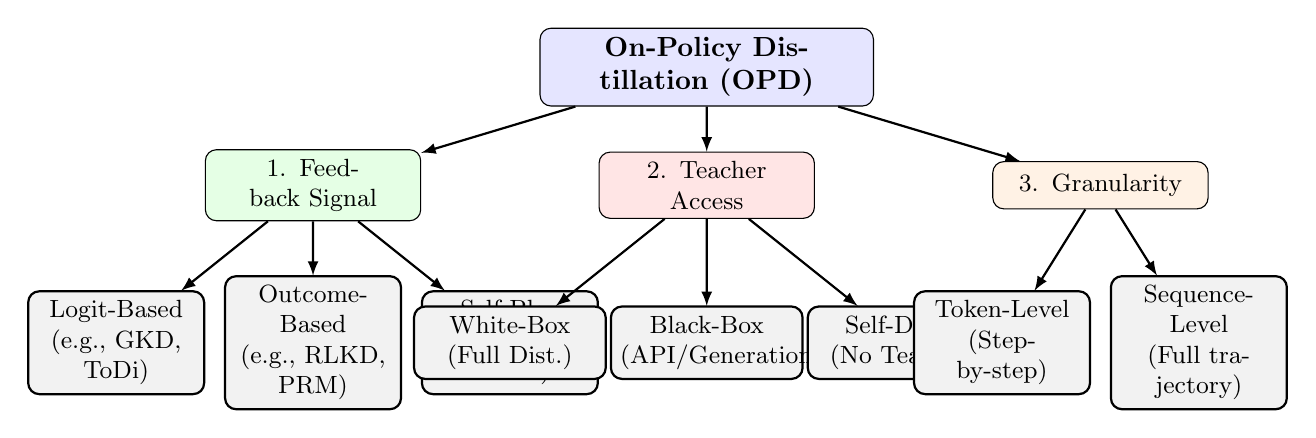
\begin{tikzpicture}[
  level 1/.style={sibling distance=5cm, level distance=1.5cm},
  level 2/.style={sibling distance=2.5cm, level distance=2cm},
  level 3/.style={sibling distance=1.5cm, level distance=2cm},
  every node/.style={rectangle, draw, rounded corners, text centered, font=\small, minimum height=0.6cm, fill=gray!10},
  edge from parent/.style={draw, -latex, thick}
]

\node [fill=blue!10, text width=4cm, font=\bfseries] {On-Policy Distillation (OPD)}
  child {node [fill=green!10, text width=2.5cm] {1. Feedback Signal}
    child {node [text width=2cm] {Logit-Based\\(e.g., GKD, ToDi)}}
    child {node [text width=2cm] {Outcome-Based\\(e.g., RLKD, PRM)}}
    child {node [text width=2cm] {Self-Play\\(e.g., SPIN, OPSD)}}
  }
  child {node [fill=red!10, text width=2.5cm] {2. Teacher Access}
    child {node [text width=2.2cm] {White-Box\\(Full Dist.)}}
    child {node [text width=2.2cm] {Black-Box\\(API/Generations)}}
    child {node [text width=2.2cm] {Self-Distill\\(No Teacher)}}
  }
  child {node [fill=orange!10, text width=2.5cm] {3. Granularity}
    child {node [text width=2cm] {Token-Level\\(Step-by-step)}}
    child {node [text width=2cm] {Sequence-Level\\(Full trajectory)}}
  };

\end{tikzpicture}
\caption{Taxonomy of On-Policy Distillation for Large Language Models. The methodology space is delineated by the nature of the feedback signal, the accessibility of the teacher's internal distributions, and the temporal granularity of the optimization objective.}
\label{fig:taxonomy_tree}
\end{figure}

\subsection{Feedback Signal: Logits, Outcomes, and Self-Play}
\label{subsec:tax_feedback}

The most critical differentiator among OPD algorithms is the nature of the supervisory signal utilized to correct the student's on-policy deviations. We partition this space into three distinct paradigms.

\textbf{Logit-Based Feedback:} In this paradigm, the student's generated sequence is evaluated token-by-token against the teacher's continuous probability distribution. Methods like GKD \citep{2306.13649} and MiniLLM \citep{2306.08543} directly compute f-divergences at every generative step. More recent advancements, such as ToDi (Trajectory-oriented Distillation) \citep{2505.16297}, optimize the alignment of token-level logits while explicitly dynamically re-weighting the importance of tokens based on their long-term impact on trajectory viability. Mathematically, logit-based feedback provides the densest possible gradient signal, as the loss vector is sized $|V|$ (the entire vocabulary) at every timestep $t$. The precise calculation inherently requires evaluating $\pteacher(\cdot|x, \hat{y}_{<t})$, ensuring the student captures the exact microscopic decision boundaries of the teacher.

\textbf{Outcome-Based Feedback:} As models scale, computing full logits becomes computationally prohibitive. Outcome-based methods abandon exact token probability matching in favor of scalar reward signals evaluating the structural validity or factual correctness of the student's generated trajectory. Frameworks like RLKD \citep{2505.16142} and approaches utilizing Process Reward Models (PRMs) \citep{2305.20050} allow the student to roll out a complete answer and then query the teacher (or a proxy reward model) for a holistic score $R(x, y)$. Optimization is typically conducted via Proximal Policy Optimization (PPO) or Direct Preference Optimization (DPO). The mathematical objective shifts from divergence minimization to reward maximization: $\max_\theta \mathbb{E}_{y \sim \ptheta} [R(x, y)] - \beta \KL(\ptheta \parallel \pi_{\mathrm{ref}})$. This provides extreme flexibility, permitting the student to find novel linguistic paths to the correct answer without being strictly tethered to the teacher's specific phrasing.

\textbf{Self-Play Feedback:} Representing the cutting edge of teacher-free alignment, self-play methodologies construct feedback signals iteratively from the student's own evolving policy. SPIN (Self-Play Fine-Tuning) \citep{2401.01335} and OPSD \citep{2601.18734} simulate a two-player game where the model at iteration $t$ attempts to distinguish its own generated trajectories from a static set of human (or teacher) demonstrations. The objective function dynamically shifts: as the student improves, the negative samples it generates become increasingly challenging, providing a naturally scaling curriculum. The loss function in SPIN elegantly pits the policy against its past iteration: $\loss(\theta) = -\mathbb{E}_{y \sim \pdata} [\log \sigma(\beta(r_\theta(x,y) - r_{\theta_{\mathrm{old}}}(x,y)))]$, strictly bounded without requiring continuous teacher intervention.

\subsection{Teacher Access: White-box, Black-box, and Self}
\label{subsec:tax_access}

The physical deployment constraints of frontier models severely limit how distillation can be practically executed. The availability of the teacher's internal states fundamentally alters the allowable mathematical formulations.

\textbf{White-Box Distillation:} When the complete weights of the teacher are accessible, algorithms can perform exact analytical divergence matching. Frameworks like DistiLLM \citep{2402.03898} leverage the full logit tensor to perform skewed KL optimizations. White-box access allows for the exploitation of dark knowledge, as the minuscule probabilities assigned to incorrect tokens carry immense structural regularization benefits. However, the memory overhead of maintaining a massive teacher (e.g., a 70B parameter model) in memory alongside the student during training requires extreme engineering optimization and immense compute clusters.

\textbf{Black-Box Distillation:} Due to the closed-source nature of frontier models (e.g., GPT-4, Claude), researchers are frequently restricted to API-level access, receiving only the hard-argmax generated text. Black-box OPD must creatively approximate the teacher distribution. Methods like Zephyr \citep{2310.06694} and Lion \citep{2310.01382} utilize the teacher purely as a preference annotator. Instead of matching $\pteacher$, the student generates multiple on-policy candidates $(y_1, y_2)$, and the black-box teacher returns a binary preference $y_1 \succ y_2$. The student then optimizes via rank-based contrastive losses. More recently, Generative Adversarial Distillation (GAD) \citep{2511.10643} attempts to implicitly model the black-box teacher's distribution by training a discriminator to differentiate between the student's on-policy text and the API's returned text, mathematically sidestepping the need for logits entirely.

\textbf{Self-Distillation:} When no superior teacher exists, the model must bootstrap its own capabilities. Self-distillation treats a stabilized, historical checkpoint of the model, or an ensembled version of itself via dropout, as the teacher. By generating responses on-policy and filtering them using its own self-evaluation mechanisms (as seen in SPIN \citep{2401.01335}), the model refines its generative manifold, correcting structural errors and smoothing its policy space without any external parameter dependencies.

\subsection{Granularity: Token, Sequence, and Trajectory}
\label{subsec:tax_granularity}

The temporal resolution at which the distillation loss is applied significantly dictates the student's ability to learn complex reasoning capabilities versus simple stylistic mimicking.

\textbf{Token-Level Granularity:} The loss is computed independently at every specific timestep $t$. The student receives immediate, localized feedback on its immediate action $y_t$. While this ensures extremely stable gradients and rapid convergence, it suffers from a pervasive myopia. A token that is mathematically improbable under the teacher's localized distribution might actually be the optimal starting token for a highly valid, alternative reasoning path.

\textbf{Sequence-Level Granularity:} The supervisory signal is applied strictly at the termination of generation. This is heavily utilized in Outcome Reward Models and methodologies focusing on end-to-end task success. While it allows the student immense freedom to explore alternative linguistic structures, the gradient signal is extremely sparse. The credit assignment problem becomes severely pronounced: if a student generates a 1000-token proof that fails at step 999, sequence-level granularity applies a uniform negative reward, failing to reinforce the 998 correct reasoning steps that preceded the error.

\textbf{Trajectory-Level (Step-by-Step) Granularity:} To resolve the dichotomy between token myopia and sequence sparsity, state-of-the-art reasoning distillation employs trajectory-level chunking. Frameworks like StepByStep \citep{2305.02301} and SuperCorrect \citep{2410.09008} utilize Process Reward Models (PRMs) \citep{2305.20050} to parse intermediate cognitive steps (e.g., separating mathematical derivations by newline delimiters). The loss is structured dynamically: $\loss = \sum_{k=1}^K \log \ptheta(s_k | s_{<k}) \cdot \hat{A}(s_k)$, where $s_k$ is a discrete chunk of the trajectory and $\hat{A}$ is the trajectory advantage. This granularity provides the precise mathematical scaffolding required to distill advanced reasoning chains from colossal models like DeepSeek-R1 down to compact architectures, achieving the delicate balance between structural freedom and rigorous logical constraint.
